% \documentclass[review]{cvpr}
\documentclass[final]{cvpr}

\usepackage{times}
\usepackage{epsfig}
\usepackage{graphicx}
\usepackage{amsmath}
\usepackage{amssymb}

% Include other packages here, before hyperref.

% If you comment hyperref and then uncomment it, you should delete
% egpaper.aux before re-running latex.  (Or just hit 'q' on the first latex
% run, let it finish, and you should be clear).
\usepackage[pagebackref=true,breaklinks=true,colorlinks,bookmarks=false]{hyperref}


\def\cvprPaperID{****} % *** Enter the CVPR Paper ID here
\def\confYear{CVPR 2021}
% \setcounter{page}{4321} % For final version only


\begin{document}

%%%%%%%%% TITLE
\title{Vision Transformer for Biomedical Image Segmentations}
\author{Bedionita Soro (20205677), Ying Hui Tan (20204871), Oh Joon Kwon (20213044)}

\maketitle

\begin{abstract}
Segmentation is crucial in biomedical images analysis for detecting diseases such as breast cancer and pulmonary diseases. However, manually detecting a specific cell or organ can be laborious and difficult because it requires professional medical knowledge. Moreover, the complexity of images (artifacts, other cells or organs) can add to errors that can be potentially harmful in medical practices. There have been numerous attempts to automate this procedure, but most recently, deep learning based automatic segmentation methods such as U-Net and its variants have gained attention. 
Nevertheless, it requires a large amount of training data, and histological images contains much noise that degrades the performance. In this paper, we exploit  recent advanced methods in deep learning and propose a multi domain approach that can semantically segment histology images for breast cancer detection and extend it to lesion segmentation in COVID-19 CT scan, exploiting domain adaptation techniques. The proposed method makes use of the recent state-of-the-art computer vision methods such as Vision Transformer (ViT). 
\end{abstract}


\section{Introduction}
Semantic segmentation is crucial in biomedical image analytics, yet requires heavy workload for manual annotation. Segmentation task can become very difficult for the pathologists even with high-expertise due to other organs, artifacts, and fatigue \cite{KRUPINSKI20061543}. This is because they often have to screen all the whole slide images (WSI) to find regions of interest with abnormal tissues or organs \cite{Randell01}. Recently, several semantic segmentation methods exploiting deep learning have been developed for histo-pathological images or organ segmentation \cite{lei2020medical}. However, most of these existing methods not only focus on a specific organ or tissue \cite{chan2019histosegnet}, but they have not largely investigated domain adaptation techniques with organs from different domains.

In this paper, we propose a semantic segmentation method with Transformer architecture \cite{vaswani2017attention} to semantically segment and identify different type of cancer regions in the WSI for breast cancer detection. We then extend this approach to segment COVID-19's lesion in lung \cite{9385788} using domain adaptation. This allows us a model to generalize over totally different domains with less effort.

\subsection{Problem and Contributions}
Organ segmentation is crucial for disease detection and treatment. Breast cancer and COVID-19 are among the common diseases that can be helped with automatic segmentation. Even though there exists some academic works on classifying cancer diseases in the WSI of breasts, those models perform below par compared to deep learning methods in computer vision. On the other hand, it is very challenging to build a model specific to that new disease due to the lack of data for COVID-19. Therefore, there is a need for domain adaptation in medical image segmentation.

The first objective of this study is to propose a deep neural network model that will efficiently and accurately identify different regions of interest in the WSI of breast for different type of cancer diseases detection. The second objective is to exploit the knowledge obtained on the breast cancer dataset to perform COVID-19 lesion segmentation through domain adaptation techniques. The performance of the proposed method will be compared with other state-of-the-art models \cite{chan2019histosegnet, chen2021transunet, Fu_2018, He2020.04.13.20063941} on publicly available datasets. The contributions of this work can be summarized as follows:
\begin{itemize}
    \item We propose a semantic segmentation method for breast cancer to identify type of regions of interest,
    \item We also investigate the problem COVID-19's lung lesion segmentation which is a hot topic with less available data. In order to address the lack of data, domain adaptation will be explored as an option, adapting histological images to the COVID-19 patient CT scans.
    \item The proposed method exploits the advantage of Vision Transformer \cite{dosovitskiy2020image}, which makes this the first work that uses Transformer in histological images segmentation for breast cancer detection,
    \item This approach will reduce the burden of manually detecting the regions of interest in histopathology images. It will provide a way to mitigate the problem of limited data in images segmentation for new diseases.
    \item We expect to compare the proposed method against some recent state-of-art methods \cite{dosovitskiy2020image,touvron2021training}.
    \item This work aims to contribute to the development of automatic healthcare systems that is becoming essential with the ongoing pandemic.
\end{itemize}

% \section{related work}

\section{Method}
The proposed method integrates recent state-of-the-art deep learning model in image classification known as Vision Transformer (ViT) \cite{dosovitskiy2020image}. Transformer, proposed by Vaswani et al.\cite{vaswani2017attention}, makes use of multi-head self-attention mechanism that can easily be scaled with large datasets. While the widely used methods in image segmentation uses convolutional neural networks (CNN) as their building blocks, parameter sharing nature of CNNs often introduces inductive bias when adapted to different data domains \cite{cohen2017inductive}. This leads to degraded model performance in these domains.

Pretrained Transformer models have been shown to be flexible when fine-tuned for down-stream tasks, both in natural language processing and computer vision. While it can be computationally expensive to pretrain the models on large datasets, Transformers often excel at adapting to different domains which makes it ideal for transfer learning and possibly domain adaptation. Moreover, the nature of semantic segmentation task requires the contextual understanding of the relationship among image regions. The self-attention mechanism that is built into Transformers could boost the model performance in such a task.

\begin{figure}[h!]
\begin{center}
% \fbox{\rule{0pt}{2in} \rule{0.9\linewidth}{0pt}}
   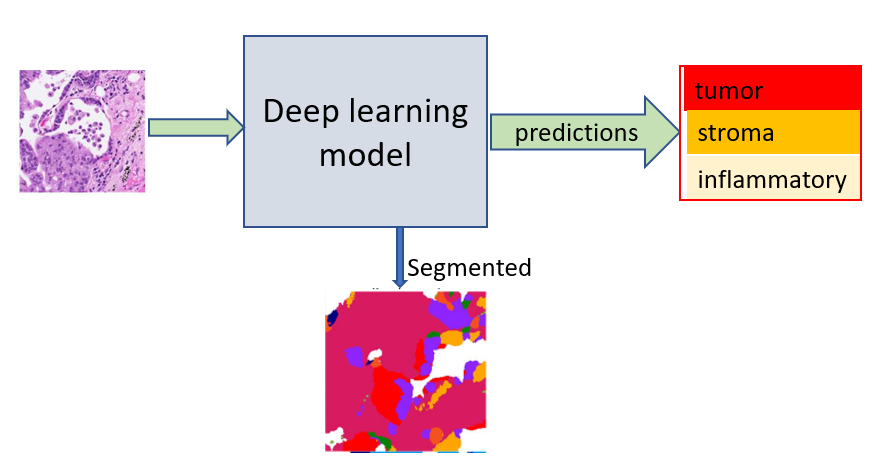
\includegraphics[width=0.8\linewidth]{media/roi1.PNG}
\end{center}
   \caption{Block diagram of the model for WSIs segmentation and classification}
\label{fig:roi}
% \label{fig:onecol}
\end{figure}

As shown in Figure \ref{fig:roi}, the first step of in this work is to build a deep learning model that will receive patches of WSIs and output the probabilities of the dominant diseases as well as the segmented version of the WSIs where each tissue type is mapped to the region of interest. Both segmentation and classification will be combined to achieve this objective. For the lung lesion segmentation, the same model will be used as a baseline. To that end, different techniques for domain adaptation will be explored such as self-supervised learning and transfer learning.

\subsection{Evaluation metric}
To evaluate the proposed method, we aim to use two different metrics for prediction and segmentation. The prediction level metric consists of: \textit{F1}, \textit{precision}, and the \textit{sensitivity} as defined in \ref{metric1}

\begin{equation}
\begin{split}
   \text{F1} & = \frac{2TP}{2TP+FP+ FN}, \\
   \text{Sensitivity} & = \frac{TP}{TP+FN}, \\
   \text{Precision} & = \frac{TP}{TP+FP} ,
   \label{metric1}
\end{split}
\end{equation}
where $TP$, $FP$ and $FN$ are true positive, false positive and false negative, respectively.

For segmentation level metric, the Jacard index or DICE's coefficient $D$ defined in equation \ref{metric2},
\begin{equation}
    D(\hat{Y},Y)=2\frac{|\hat{Y} \cap Y|}{|\hat{Y} \cup Y|},
    \label{metric2}
\end{equation}
where $\hat{Y}$ and $Y$ are the predicted region from the model and the ground truth region of input image, respectively.

\section{Data}
The model will be trained and assessed on several datasets. The first dataset used in this study was introduced in \cite{10.1093/bioinformatics/btz083}. It consists of 151 hematoxylin and eosin strained whole-slide images (WSIs) from histologically confirmed cases of breast cancer. The dataset is available on the Cancer Genome Atlas. The mean and the standard deviation of the region of interest are respectively 1.18mm\textsuperscript{2} and 0.80mm\textsuperscript{2}. The second dataset considered is from \cite{zhao2020COVID-CT-Dataset} which consists of 349 COVID-19 CT images from 216 patients and 463 non-COVID-19 CTs. In addition to that we will used another publicly available dataset published by China National Center for Bioinformation \cite{Gunraj2020} consisting of 650 scans across 150 patients with various stages of COVID.

\newpage 
\section{Tentative plan}
\begin{figure}[h!]
\begin{center}
% \fbox{\rule{0pt}{2in} \rule{0.9\linewidth}{0pt}}
   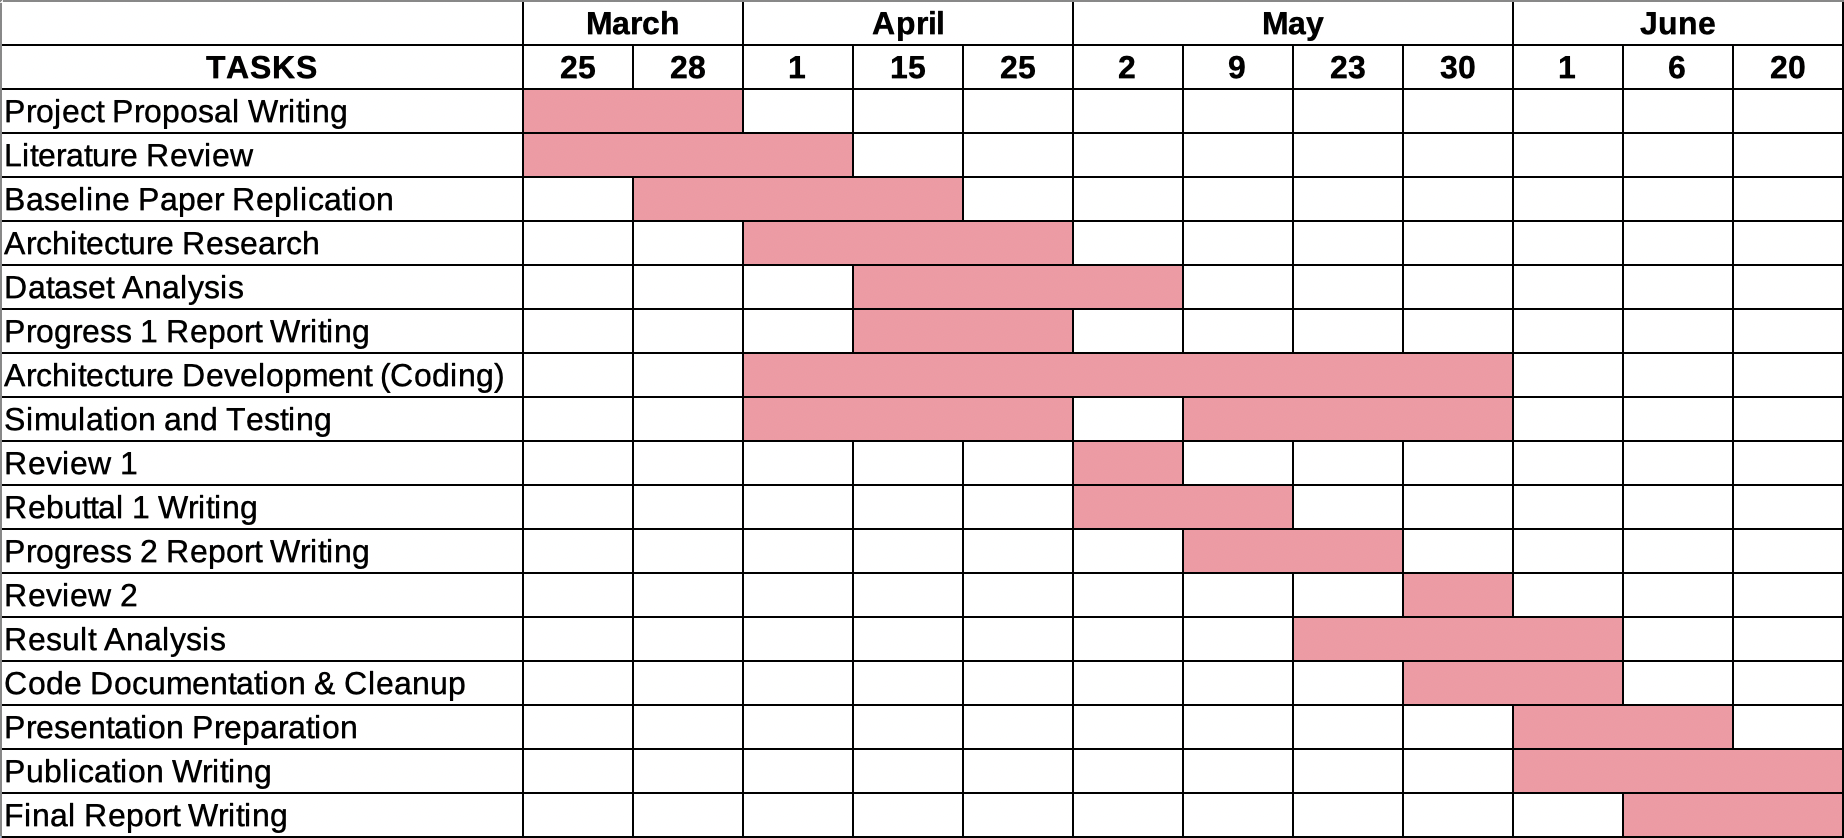
\includegraphics[width=1.0\linewidth]{media/chart.png}
\end{center}
   \caption{Tentative schedule}
\label{fig:schedule}
% \label{fig:onecol}
\end{figure}

%\cite{Randell}.
% \cite{10.1093/bioinformatics/btz083}

% \section{Guideline: Progress 1 / 2}

% After the proposal, we will check the progress of your project two times. You should submit the progress reports, and the reports should contain the contents of the proposal, \textit{related work} (and \textit{previous work} if exist), \textit{method}, and \textit{experiment}. It is okay to omit the result.

% Other students will review your progress reports, and it is in a fully \textit{double-blind} manner. Each team will receive three or four reviews, and the review scores will affect your final score. For fair evaluation, students who have the same advisor do not review each others' work, and also \textbf{you will judge the reviews' review!} In the case of Progress 1, every team should submit \textit{author response}. The length of the response is up to one page. We provide the template for the author response; please check \texttt{01\_rebuttal.tex}.

% \section{Guideline: Final}

% The final report should contain the contents of the proposal and the progress reports, \textit{result}, and \textit{etc}. The length of the paper is up to nine pages except for \textit{reference}. Reference is optional, but we strongly recommend you to add the reference.

% There will be a project presentation session at the end of the semester. Further instructions will be announced later.

% \section{Etc}

% If you have a question, send us an e-mail or a message to the Kakao open chat room.

{\small
\bibliographystyle{ieee_fullname}
\bibliography{reference}
}

\end{document}
